\subsection{During Training}
\begin{figure}[ht]
	\centering
	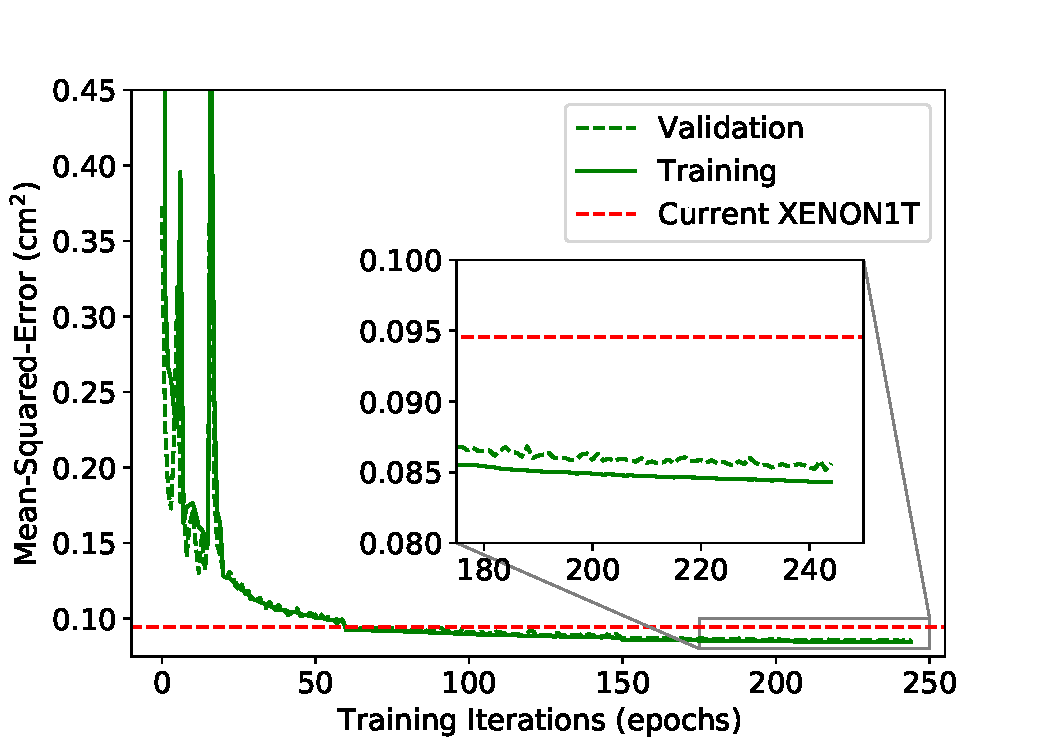
\includegraphics[width=0.8\linewidth]{figures/del_mse-v-epo_insetted.pdf}
	\caption{Mean squared error (MSE) in square centimeters of the GCNN for the training set and validation set during the training process.
	The minimum MSE for the MLP is given in red at 0.0945 cm\textsuperscript{2}. This is the benchmark that the GCNN has to pass during training.
	Spikes within the first 20 epochs occur due to large step size during gradient descent.
	This was temporary solved by lowering the step size at epochs 20, 60, and 150.
	These milestones were placed by observations of previous trainings, but the permanent solution will be based on the MSE as it's training.
	The minimum MSE achieved by our GCNN on the validation set is 0.0852 cm\textsuperscript{2}.}
	\label{fig:GCNN_Training}
\end{figure}
The performance of our GCNN was compared to a MLP during training as a benchmark and early warning system.
If the GCNN did not approach a comparable performance to that of the MLP swiftly enough, training would typically stagnate and not surpass this benchmark.
By not performing better than the MLP here, it was generally indicative that the GCNN would also perform worse when we gave attention to our performance metrics.
After a few iterations of this, we chose to only look at the performance metrics if the GCNN model produced a lower MSE during training and would restart training in cases where it was clear that the GCNN would not perform better within a reasonable number of epochs.
An example of when it was clear the GCNN would not do better is if the MSE was not below $0.25$ cm\textsuperscript{2} within the first $50$ epochs.
\begin{wrapfigure}{r}{0.5\textwidth}
	\centering
	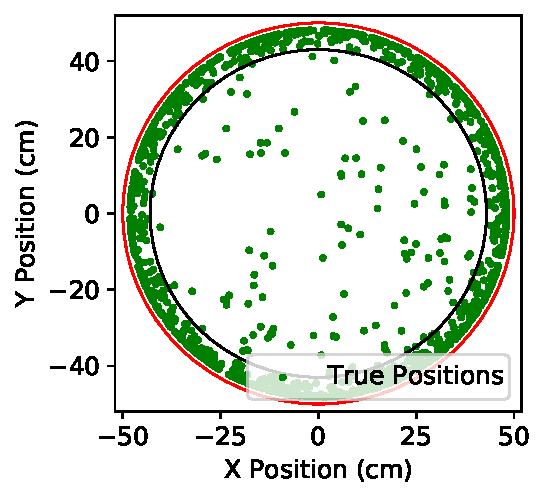
\includegraphics[width=\linewidth]{figures/gcnn_Delaunay-Prenoise_1cm-err.pdf}
	\caption{
	True positions of GCNN mis-reconstructions.
	Only 1680 of the 197,975 simulated events were mis-reconstructed and are shown here.
	Red circle is the wall of the detector (50 cm); black circle is the largest radius of the fiducial volume (43 cm).
	It's clear that the majority of these mis-reconstructions occur near the wall and are beyond the largest radius of the fiducial volume.
	Only 123 of the 1680 mis-reconstructions are within the fiducial volume.
	}
	\label{fig:1cm_Counts}
\end{wrapfigure}
\par We used an optical Monte Carlo simulation for training as an attempt to assume a “perfect” detector.
This is to say that no spurious events, such as single electrons, dark counts, or PMT after-pulses, were within our simulation.
The observations by the PMTs are as if every part of the detector ran perfectly.
By using a simulation like this, we were able to input the data into our model without normalization or standardization.
\par The GCNN was able to outperform the MLP in training, which is a good indicator for the overall performance.
Much of the work for this stage was in optimizing the learning rate used for gradient descent.
Our solution was to lower the learning rate  at specific epochs based on the performance of  previous results.
We ended up lowering the learning rate at epochs 20, 60, and 150.
This caused notable bumps within Figure \ref{fig:GCNN_Training} and resulted in a much smoother curve after epoch 20.
However, a better solution would have the learning rate lower based on the GCNN's performance during training instead of milestones set by the attentive user.
\subsection{Validation Set Performance}
As previously stated, the two performance metrics we focused on are to have no reconstructions outside the detector and to minimize the number of reconstructions that are 1 cm away from the true position.
For best practice in machine learning, we focused on the results of the validation set which is made of 197,975 simulated events.
\begin{figure}[t]
	\centering
	\begin{subfigure}[b]{0.45\textwidth}
		\centering
		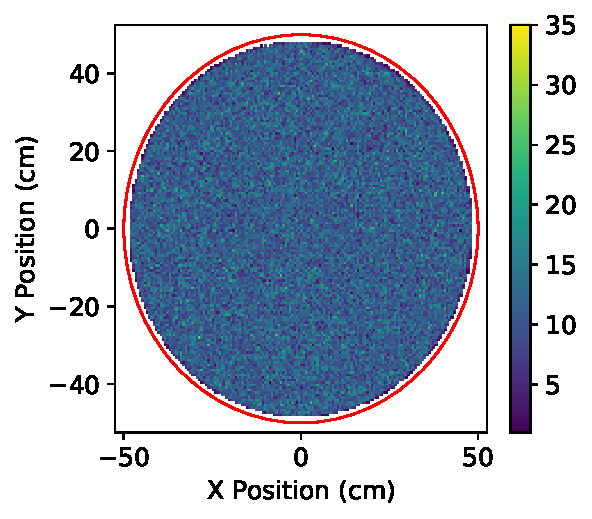
\includegraphics[width=\textwidth]{figures/optsim_val_true_pos.pdf}
	\end{subfigure}
	\hfill
	\begin{subfigure}[b]{0.45\textwidth}
		\centering
		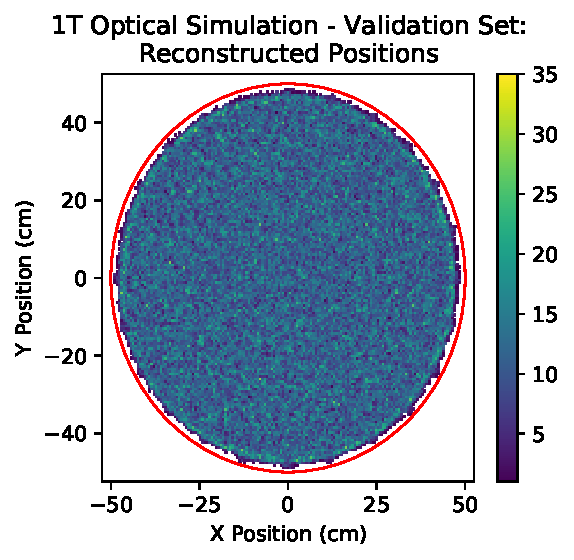
\includegraphics[width=\textwidth]{figures/optsim_val_reco_pos.pdf}
	\end{subfigure}
	\caption{
	2D histograms of the true positions and reconstructed positions at 150 bins.
	Red circle is the wall of the detector (50 cm).
	The edge of the reconstructed positions is notably jagged, but entirely contained within the walls of the detector.
	This agrees with our expectations of doing poorly near the wall of the detector while still succeeding in containing the reconstructions within the detector.
	Otherwise, the uniform reconstruction is a good indicator that there aren't any particular spots of inaccuracy nor is there any outstanding inward reconstruction bias.
	}
	\label{fig:2D_Hists}
\end{figure}
\par Since we are hard set on having no reconstructions outside of the detector, this was the first metric we would check.
As it turned out, we counted zero reconstructions outside of the detector for our latest version of the GCNN.
At this point, our GCNN has successfully surpassed the MLP training benchmark and made no exceedingly erroneous reconstructions, a rule that previous implementations had difficulty passing.
\par As for the further than 1 cm reconstructions, these too performed well.
Only 1680 of the 197,975 events were reconstructed at greater than 1 cm away from the true position.
That is about 0.85\% of the validation set.
As can be seen in Figure \ref{fig:1cm_Counts}, many of the mistakes are made along the walls of the detector and explained the jagged edge found in Figure \ref{fig:2D_Hists}.
If we reduce the area we count on to the maximum radius of the fiducial volume ($R=43$ cm), we find only 123 of the 197,975 events mis-reconstructed.
Only 0.06\% of the validation set!
\par The last important performance check, as for any experiment, is to produce the most accurate measurements or reconstructions, in our case.
For this we use the resolution metrics $\Delta X$, $\Delta Y$, and $\Delta R$:
\begin{gather*}
	\Delta X \equiv X_\text{Reconstructed} - X_\text{Simulated},
	\quad \Delta Y \equiv Y_\text{Reconstructed} - Y_\text{Simulated}, \\
	\quad \Delta R \equiv \sqrt{ \Delta X^2 + \Delta Y^2 }
\end{gather*}
where $X$ and $Y$ are the $x$ and $y$ positions of the reconstructions and the associated simulation.
As for the means and standard deviations produced by our GCNN are shown in Figure \ref{fig:1D_Hist}.
We found $\Delta X$ with a mean of -0.00578 cm and standard deviation of 0.292 cm, $\Delta Y$ with a mean of -0.00536 cm and standard deviation of 0.291 cm, and $\Delta R$ with a mean of 0.346 cm and a standard deviation of 0.224 cm.
This too outperformed the MLP which had standard deviations greater than 3 cm.
From previous observations of the results of our GCNN, the mean and standard deviation of $\Delta R$ follows suit with what we expect: most of the reconstructions are within 1 cm of the true, simulated position.
At the same time, the approximately-Gaussian curves of $\Delta X$ and $\Delta Y$ further confirms the positive performance of our GCNN.
\begin{figure}[t]
	\centering
	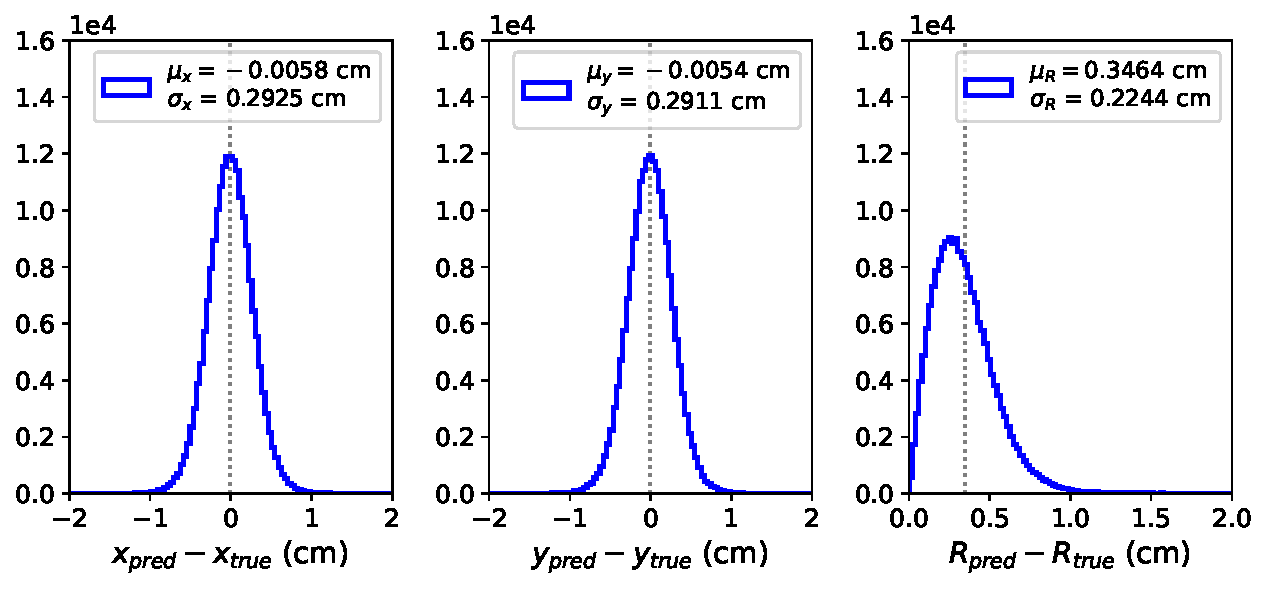
\includegraphics[width=0.9\linewidth]{figures/1D_hist_Delaunay-Prenoise.pdf}
	\caption{
	1D histograms of the reconstructed position minus the true positions.
	There are 100 bins between -2 cm and 2 cm on $\Delta X, \Delta Y$ and 100 bins between 0 cm and 3 cm on $\Delta R$.
	For $\Delta X$ we achieved a mean value of -0.00578 cm and a standard deviation of 0.292 cm.
	For $\Delta Y$ we achieved a mean value of -0.00536 cm and a standard deviation of 0.291 cm.
	For $\Delta R$ we achieved a mean value of 0.346 cm and a standard deviation of 0.224 cm.
	Both the $\Delta X$ and $\Delta Y$ histograms are near Gaussian curves of the same statistics.
	}
	\label{fig:1D_Hist}
\end{figure}
